\documentclass{article}
\usepackage{amsmath}
\usepackage{amsthm}
\usepackage{amsfonts}
\usepackage{amssymb}
\usepackage{bbold}
\usepackage{dsfont}
\usepackage{graphicx}
\usepackage{cleveref}
\usepackage{bm}
\usepackage{booktabs}
\usepackage{siunitx}
\usepackage{xcolor}
\usepackage{pdfpages}
\usepackage[utf8]{inputenc}
\usepackage[english]{babel}
\newtheorem{definition}{Definition}
\newtheorem{example}{Example}
\newcommand{\exP}[1]{\mathrm{e}^{#1}}
\newcommand{\dif}{\mathrm{d}}
\renewcommand{\vec}[1]{\mathbf{#1}}
\newcommand{\pdagger}{{\phantom{\dagger}}}
\newcommand{\state}[1]{\vert #1\rangle}
\newcommand{\cstate}[1]{\langle #1\vert}
\newcommand{\tr}[1]{\mathrm{tr}\left\{#1\right\}}
\newcommand{\trs}[2]{\, \mathrm{tr}_{#1}\{#2\}}
\newcommand{\expc}[3]{\langle #1\vert #2 \vert #3\rangle}
\usepackage[doi=false,url=false,isbn=false,backend=bibtex,style=nature,natbib=true,sorting=none]{biblatex}
\bibliography{bib.bib}
\usepackage{geometry}
\geometry{
	a4paper,
	total={170mm,257mm},
	left=15mm,
	right=15mm,
	top=15mm,
}
\begin{document}
\title{Transport through spinfull Peierls model with tAMEn algorithm}
\maketitle

\section{Model}
The model is a junction, split into system, bath and interaction terms
\begin{equation}
	H = H_S + H_B + H_I
\end{equation}  
The system consists of a chain of electronic levels with bare energy $\varepsilon_0$ and nearest-neighbor electronic hopping $t_0$ and Peierls-type electron-vibrational coupling $\lambda$ to harmonic oscillator modes with frequency $\omega_0$
\begin{equation}
	H_S = \varepsilon_0 \sum_{j\sigma}  d^\dagger_{j\sigma} d_{j\sigma}^\pdagger + \omega_0 \sum_j a_j^\dagger a_j^\pdagger + \sum_{j\sigma} (d_{j\sigma}^\dagger d_{j+1,\sigma} + \mathrm{h.c.})( -t_0 + t_1(a_j^\dagger + a_j)).
\end{equation}
The bath are two electrodes $\ell=L,R$, modeled as free electrons
\begin{equation}
	H_B = \sum_{k\ell} \varepsilon_{k\ell}c^\dagger_{k\ell}c^\pdagger_{k\ell}
\end{equation}
and the system-bath coupling is linear in system and bath operators
\begin{equation}
	H_I = \sum_{k_L, k_R,\sigma} (V_{k_L,\sigma} c_{k_L,\sigma}^\dagger d_{1,\sigma} + V_{k_R} c_{k_R,\sigma}^\dagger d_{N,\sigma}  + \mathrm{h.c.}),
\end{equation}
where $N$ is the number of electronic sites. The molecule-lead coupling is characterized by the line-width function
\begin{equation}
	\Gamma_\ell(\varepsilon) = 2\pi\sum_{k_\ell, ,\sigma} V_{k_\ell,\sigma}V_{k_\ell,\sigma}^* \delta(\varepsilon-\varepsilon_{k_\ell,\sigma}) \equiv \mathrm{const},
\end{equation}
which is assumed to be constant (wide-band limit). Electrons are assumed spin-less in this model.
\section{Parameters}
The parameters of the model above are listed as follows
\begin{align*}
	\varepsilon_0 &= -\SI{240}{\milli\electronvolt}\\
	\hbar \omega_0 &= \SI{2}{\milli\electronvolt}\\
	t_0 &= \SI{40}{\milli\electronvolt}\\
	t_1 &=\SI{4}{\milli\electronvolt}\\ 
	\Gamma_\ell &= \SI{10}{\milli\electronvolt}\\
	k_B T_\ell &= \SI{0.026}{\electronvolt}\\ 
	W&=\mathrm{WBL}.
\end{align*}
\clearpage
\section{Results}
\begin{figure}[!h]
	\centering
	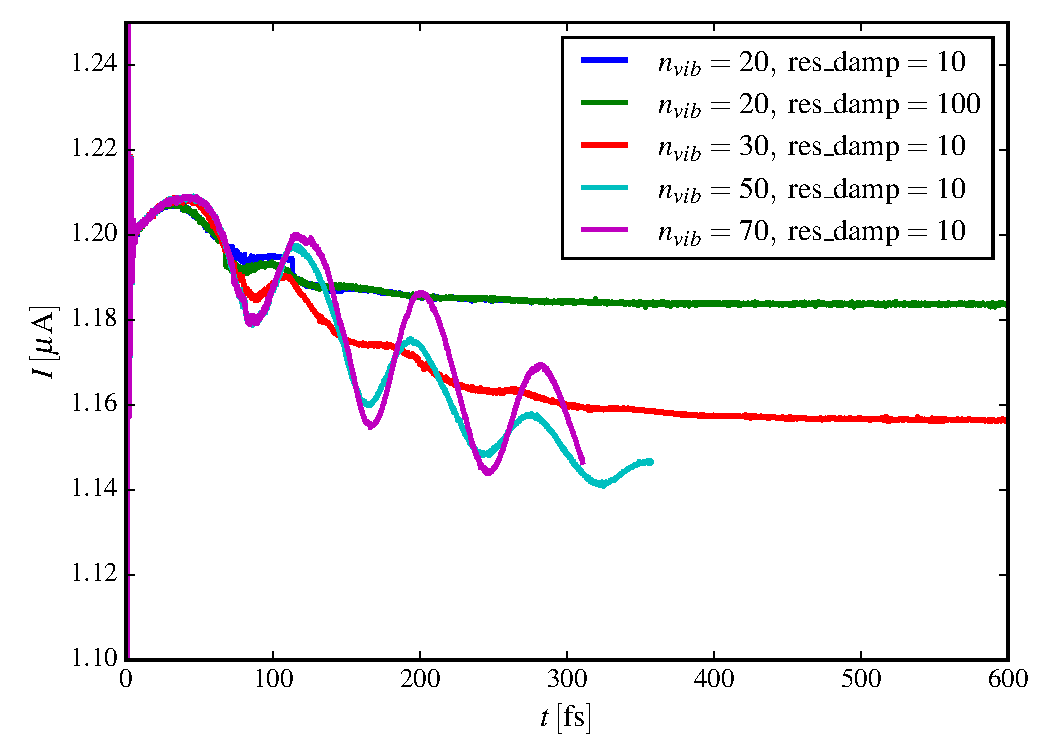
\includegraphics[width=0.8\textwidth]{figs/Peierls_L2_spin_V60_mvibVar_currents.pdf}
\end{figure}
\begin{figure}[!h]
	\centering
	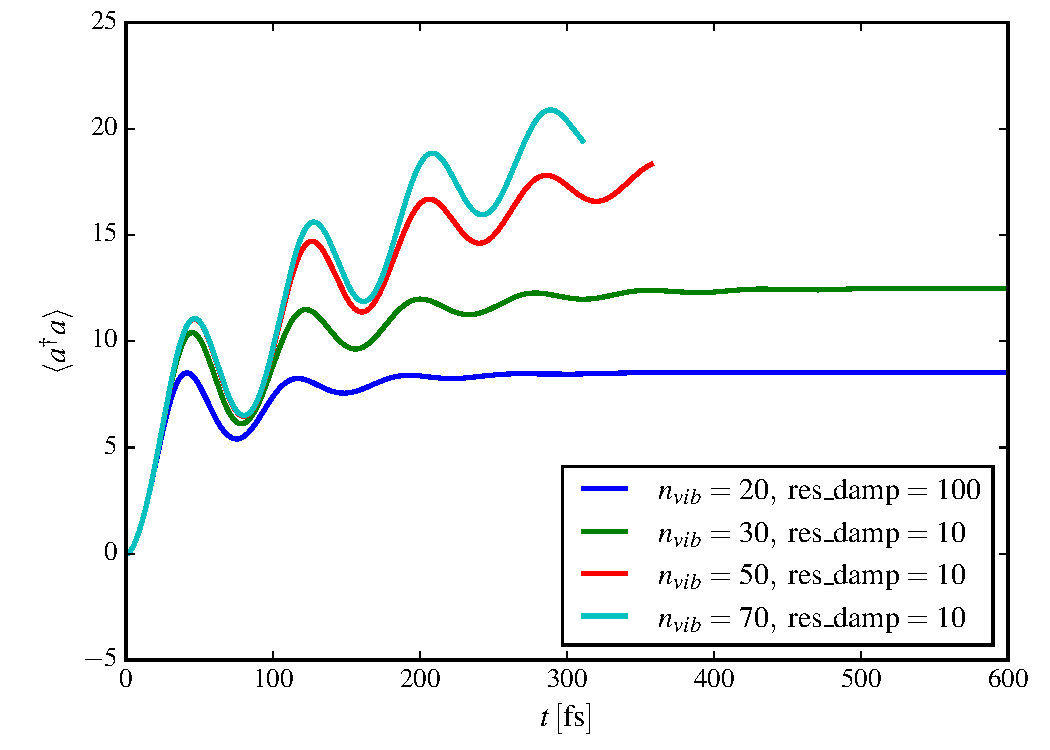
\includegraphics[width=0.8\textwidth]{figs/Peierls_L2_spin_V60_mvibVar_nvib.pdf}
\end{figure}
\begin{figure}[!h]
	\centering
	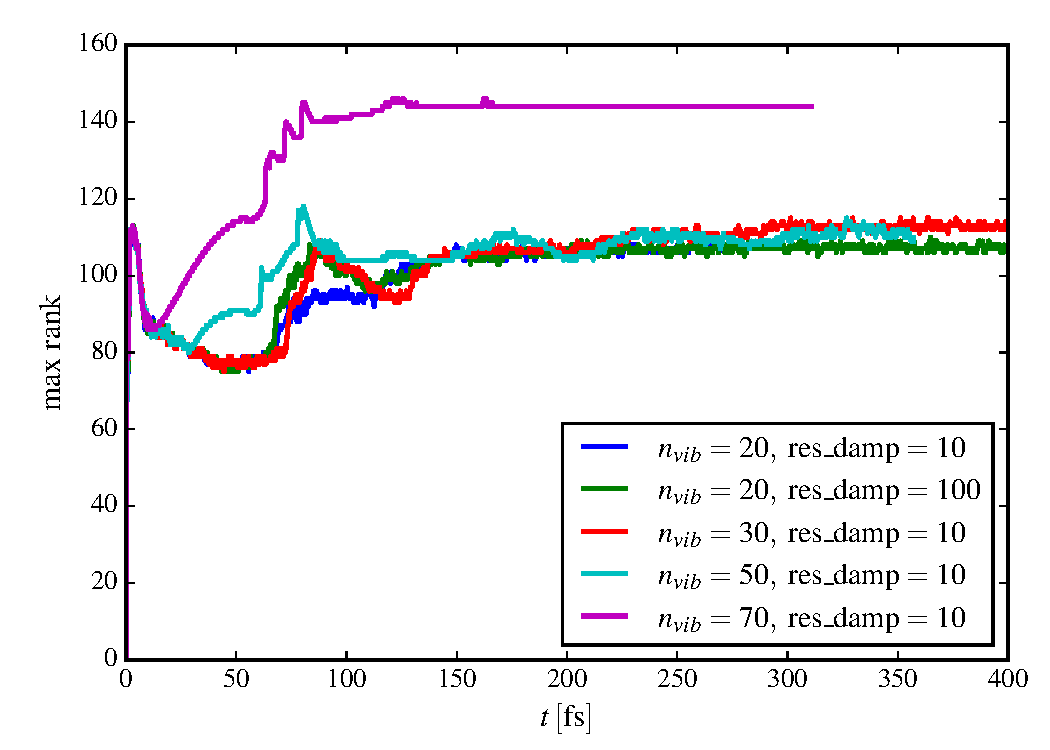
\includegraphics[width=0.8\textwidth]{figs/Peierls_L2_spin_V60_mvibVar_max_rank.pdf}
	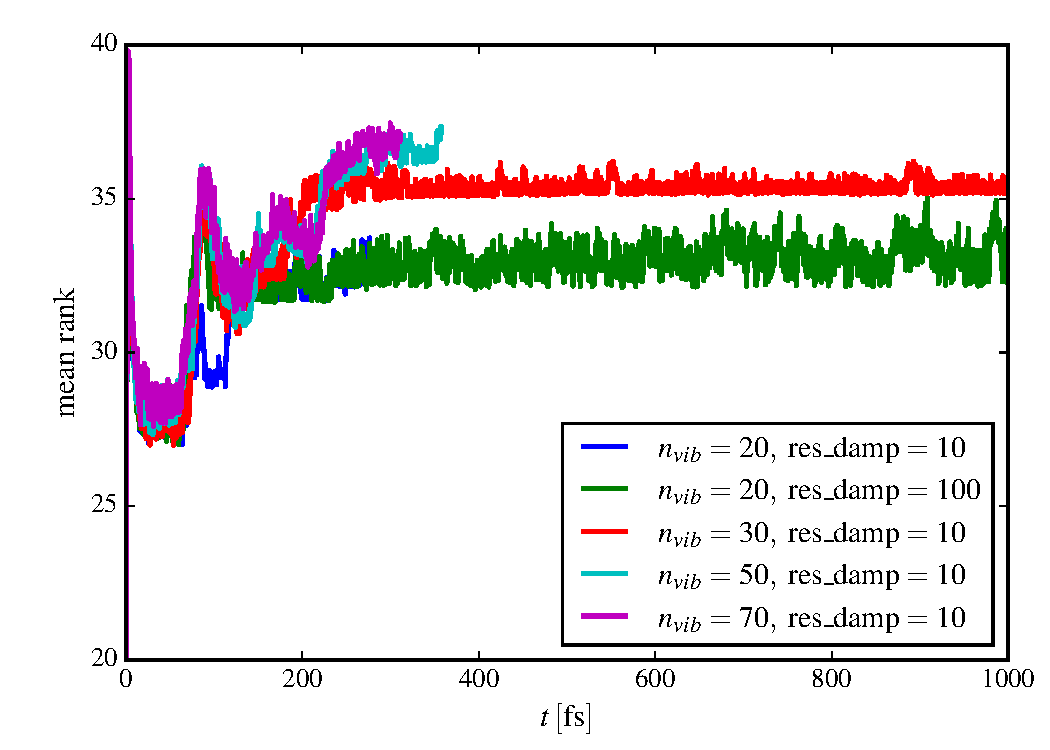
\includegraphics[width=0.8\textwidth]{figs/Peierls_L2_spin_V60_mvibVar_mean_rank.pdf}
\end{figure}

\clearpage


\end{document}


